\documentclass{article}

\usepackage[utf8]{inputenc}
\usepackage{graphicx}
\usepackage{amsmath}
\usepackage[hidelinks]{hyperref}

\title{Connect 4 Writeup}
\author{Dylan Ang}
\date{\today}

\begin{document}

\maketitle

\tableofcontents

    
\section{Question 1: Evaluation Function}

\subsection{Part A}

My evaluation function assigns a score to a state by checking if a given cell is occupied by player 1 or 2, and adding or a subtracting from a score total accordingly. 
The actual amounts added or subtracted from the score for occupied cells depends on which cell. 
On a connect 4 board, there are 69 ways to win, and some cells within the board are in multiple winning lines.
For example, the bottom left corner of the board can be a part of 3 different winning lines, the vertical, diagonal, and horizontal lines.
We can say then that if we took the bottom left corner of the board, 
I have a matrix in which the value in each cell corresponds to the number of lines of length 4 that pass through it.
In my evaluation function I iterate through the board, and if the current cell is our player, I add the value of that same cell in the weight matrix from the score.
If the current cell holds our opponent, I subtract the value of the cell in the weight matrix from the score.

\subsection{Part B}

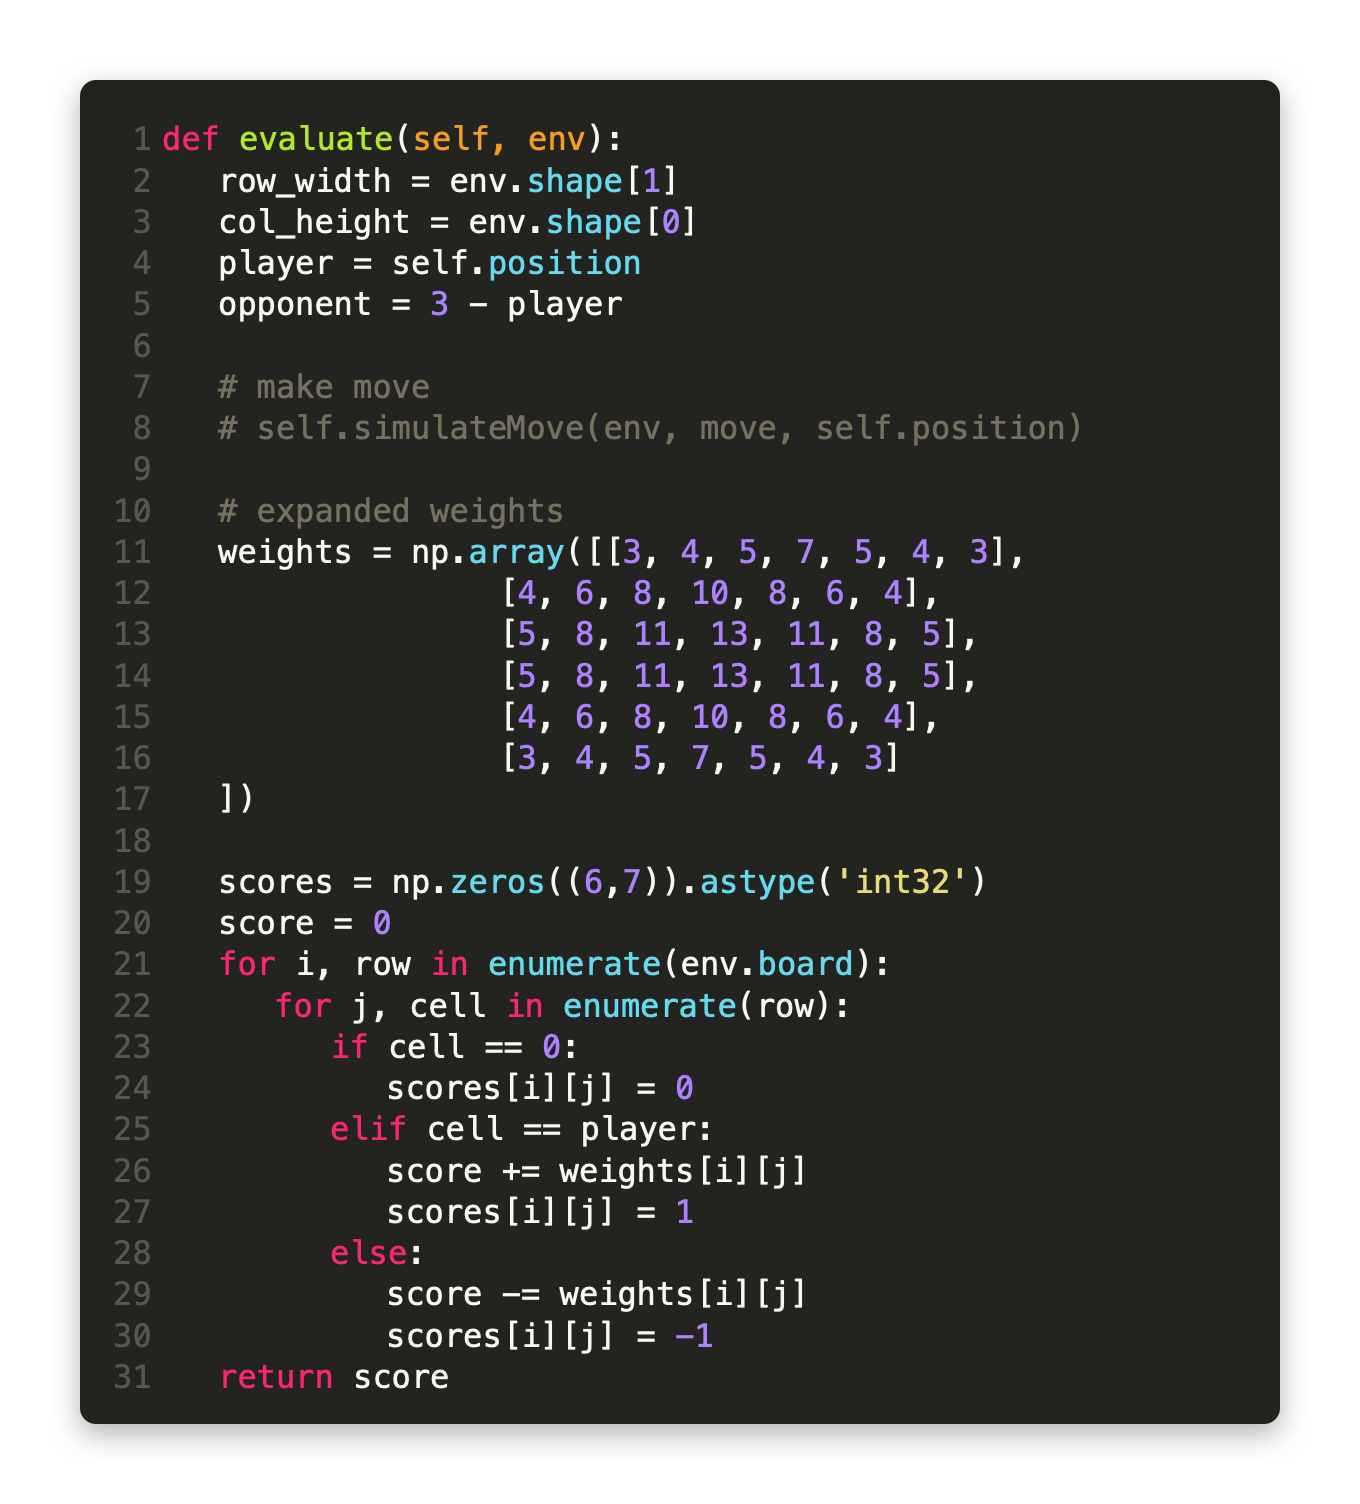
\includegraphics[width = \linewidth]{codye.png}

\subsection{Part C}

For a given board configuration A,
\begin{equation*}
    A = \left[ \begin{matrix}
        0 & 0 & 0 & 0 & 2 & 0 & 0 \\
        0 & 0 & 0 & 1 & 1 & 0 & 0 \\
        0 & 0 & 2 & 2 & 1 & 0 & 0 \\
        0 & 0 & 1 & 1 & 1 & 0 & 0 \\
        0 & 0 & 2 & 1 & 2 & 0 & 0 \\
        0 & 0 & 2 & 1 & 2 & 0 & 0 \\
    \end{matrix} \right]
\end{equation*}

We compare it to our weight matrix.
\begin{equation*}
    W = \left[ \begin{matrix}
        3 & 4 & 5 & 7 & 5 & 4 & 3 \\
        4 & 6 & 8 & 10 & 8 & 6 & 4 \\
        5 & 8 & 11 & 13 & 11 & 8 & 5 \\
        5 & 8 & 11 & 13 & 11 & 8 & 5 \\
        4 & 6 & 8 & 10 & 8 & 6 & 4 \\
        3 & 4 & 5 & 7 & 5 & 4 & 3 \\
    \end{matrix} \right]
\end{equation*}

\begin{align*}
A.weight & = ((10 + 8) + (11) + (11 + 13 + 11) + (10) + (7)) \\
         & + (-1) * ((5) + (11 + 13) + (8 + 8) + (5 + 5)) \\
         & = 81 - 55 \\
         & = 26 
\end{align*}

\section{Question 2}

Find implementation in players.py

\section{Question 3}

\begin{verbatim}
Minimax Games

===== Minimax VS Stupid =====

Summary: 
p1 Wins: 5
p2 Wins: 0

> python main.py -p1 minimaxAI -p2 stupidAI -limit_players 1,2 -seed 1 
[[0 0 0 2 0 0 0]
    [0 0 0 1 0 0 0]
    [0 0 0 2 0 0 0]
    [0 0 2 1 0 0 0]
    [0 0 2 2 0 0 0]
    [1 1 1 1 0 0 0]]
Player  1  has won

> python main.py -p1 minimaxAI -p2 stupidAI -limit_players 1,2 -seed 2
[[0 0 0 2 0 0 0]
    [0 0 0 1 0 0 0]
    [0 0 0 2 0 0 0]
    [0 0 2 1 0 0 0]
    [0 0 2 2 0 0 0]
    [1 1 1 1 0 0 0]]
Player  1  has won

> python main.py -p1 minimaxAI -p2 stupidAI -limit_players 1,2 -seed 3 
[[0 0 0 2 0 0 0]
    [0 0 0 1 0 0 0]
    [0 0 0 2 0 0 0]
    [0 0 2 1 0 0 0]
    [0 0 2 2 0 0 0]
    [1 1 1 1 0 0 0]]
Player  1  has won

> python main.py -p1 minimaxAI -p2 stupidAI -limit_players 1,2 -seed 4 
[[0 0 0 2 0 0 0]
    [0 0 0 1 0 0 0]
    [0 0 0 2 0 0 0]
    [0 0 2 1 0 0 0]
    [0 0 2 2 0 0 0]
    [1 1 1 1 0 0 0]]
Player  1  has won

> python main.py -p1 minimaxAI -p2 stupidAI -limit_players 1,2 -seed 5 
[[0 0 0 2 0 0 0]
    [0 0 0 1 0 0 0]
    [0 0 0 2 0 0 0]
    [0 0 2 1 0 0 0]
    [0 0 2 2 0 0 0]
    [1 1 1 1 0 0 0]]
Player  1  has won

===== Stupid VS Minimax =====

Summary: 
p1 Wins: 0
p2 Wins: 5

> python main.py -p1 stupidAI -p2 minimaxAI -limit_players 1,2 -seed 1
[[0 0 1 2 0 0 0]
    [0 0 1 1 0 0 0]
    [0 0 2 2 0 0 0]
    [0 0 1 1 0 0 0]
    [0 2 2 2 2 0 0]
    [0 1 1 1 2 0 0]]
Player  2  has won

> python main.py -p1 stupidAI -p2 minimaxAI -limit_players 1,2 -seed 2
[[0 0 1 2 0 0 0]
    [0 0 1 1 0 0 0]
    [0 0 2 2 0 0 0]
    [0 0 1 1 0 0 0]
    [0 2 2 2 2 0 0]
    [0 1 1 1 2 0 0]]
Player  2  has won

> python main.py -p1 stupidAI -p2 minimaxAI -limit_players 1,2 -seed 3
[[0 0 1 2 0 0 0]
    [0 0 1 1 0 0 0]
    [0 0 2 2 0 0 0]
    [0 0 1 1 0 0 0]
    [0 2 2 2 2 0 0]
    [0 1 1 1 2 0 0]]
Player  2  has won

> python main.py -p1 stupidAI -p2 minimaxAI -limit_players 1,2 -seed 4
[[0 0 1 2 0 0 0]
    [0 0 1 1 0 0 0]
    [0 0 2 2 0 0 0]
    [0 0 1 1 0 0 0]
    [0 2 2 2 2 0 0]
    [0 1 1 1 2 0 0]]
Player  2  has won

> python main.py -p1 stupidAI -p2 minimaxAI -limit_players 1,2 -seed 5
[[0 0 1 2 0 0 0]
    [0 0 1 1 0 0 0]
    [0 0 2 2 0 0 0]
    [0 0 1 1 0 0 0]
    [0 2 2 2 2 0 0]
    [0 1 1 1 2 0 0]]
Player  2  has won

===== Minimax VS Random =====

Summary: 
p1 Wins: 5
p2 Wins: 0

> python main.py -p1 minimaxAI -p2 randomAI -limit_players 1,2 -seed 1
[[0 0 0 2 0 0 0]
    [0 0 0 1 0 0 0]
    [0 0 0 2 0 0 0]
    [0 0 0 1 0 0 0]
    [2 0 0 1 0 0 0]
    [2 2 1 1 1 1 2]]
Player  1  has won

> python main.py -p1 minimaxAI -p2 randomAI -limit_players 1,2 -seed 2
[[0 0 0 0 0 0 0]
    [0 0 0 0 0 0 0]
    [0 0 0 1 0 0 0]
    [0 0 0 1 0 0 0]
    [0 0 0 1 0 0 0]
    [2 0 2 1 0 2 0]]
Player  1  has won

> python main.py -p1 minimaxAI -p2 randomAI -limit_players 1,2 -seed 3
[[0 0 0 0 0 0 0]
    [0 0 0 0 0 0 0]
    [0 0 0 1 0 0 0]
    [0 0 0 1 2 0 0]
    [0 0 0 1 2 0 0]
    [0 0 0 1 2 0 0]]
Player  1  has won

> python main.py -p1 minimaxAI -p2 randomAI -limit_players 1,2 -seed 4
[[1 0 0 1 0 0 0]
    [2 0 0 1 0 0 0]
    [1 0 0 1 0 0 0]
    [2 0 0 2 2 0 0]
    [2 1 1 1 1 0 0]
    [2 2 2 1 2 0 0]]
Player  1  has won

> python main.py -p1 minimaxAI -p2 randomAI -limit_players 1,2 -seed 5
[[0 0 0 0 0 0 0]
    [0 0 0 0 0 0 0]
    [0 0 0 1 0 0 0]
    [0 0 0 1 0 2 0]
    [0 0 0 1 0 2 0]
    [0 0 0 1 0 2 0]]
Player  1  has won

===== Random VS Minimax =====

Summary: 
p1 Wins: 0
p2 Wins: 5

> python main.py -p1 randomAI -p2 minimaxAI -limit_players 1,2 -seed 1
[[0 0 0 1 0 0 0]
    [0 0 0 2 0 0 0]
    [0 0 0 1 2 0 0]
    [0 0 0 2 1 0 1]
    [2 0 2 2 1 0 1]
    [1 2 2 2 1 0 1]]
Player  2  has won

> python main.py -p1 randomAI -p2 minimaxAI -limit_players 1,2 -seed 2
[[0 0 0 0 0 0 0]
    [0 0 0 0 0 0 0]
    [0 0 0 2 0 0 0]
    [0 0 0 2 0 0 0]
    [0 0 0 2 0 0 0]
    [1 1 0 2 0 1 1]]
Player  2  has won

> python main.py -p1 randomAI -p2 minimaxAI -limit_players 1,2 -seed 3
[[0 0 0 0 0 0 0]
    [0 0 0 0 0 0 0]
    [0 0 0 2 0 0 0]
    [0 0 0 2 0 0 0]
    [0 0 0 2 1 0 0]
    [0 0 1 2 1 1 0]]
Player  2  has won

> python main.py -p1 randomAI -p2 minimaxAI -limit_players 1,2 -seed 4
[[0 0 0 2 0 0 0]
    [0 0 0 1 0 0 0]
    [0 0 0 2 0 0 0]
    [2 2 2 2 0 0 0]
    [1 1 2 1 0 0 0]
    [1 1 1 2 0 1 0]]
Player  2  has won

> python main.py -p1 randomAI -p2 minimaxAI -limit_players 1,2 -seed 5
[[0 0 0 0 0 0 0]
    [0 0 0 0 0 0 0]
    [0 0 0 2 0 0 0]
    [0 0 0 2 0 0 0]
    [0 0 0 2 0 0 0]
    [1 0 1 2 0 1 1]]
Player  2  has won

===== Minimax VS MonteCarlo =====

Summary:
p1 Wins: 7
p2 Wins: 3

> python main.py -p1 minimaxAI -p2 monteCarloAI -limit_players 1,2 -seed 1
[[2 0 1 1 1 0 0]
    [2 0 1 1 1 0 0]
    [1 0 1 1 1 0 0]
    [2 0 2 2 2 1 1]
    [2 0 1 1 2 2 2]
    [2 2 2 1 2 1 2]]
Player  1  has won

> python main.py -p1 minimaxAI -p2 monteCarloAI -limit_players 1,2 -seed 2
[[1 2 0 2 1 0 0]
    [2 1 0 1 1 0 0]
    [1 1 0 1 1 0 0]
    [2 1 2 2 2 2 0]
    [1 2 2 1 2 1 0]
    [2 2 1 1 2 2 0]]
Player  2  has won

> python main.py -p1 minimaxAI -p2 monteCarloAI -limit_players 1,2 -seed 3
[[0 0 0 1 0 1 0]
    [0 0 2 1 0 1 0]
    [0 0 1 1 2 1 0]
    [0 0 1 2 1 1 0]
    [1 0 2 1 2 2 2]
    [2 0 2 1 2 2 2]]
Player  1  has won

> python main.py -p1 minimaxAI -p2 monteCarloAI -limit_players 1,2 -seed 4
[[1 2 1 1 2 0 2]
    [1 2 1 1 2 0 1]
    [1 1 1 2 1 0 2]
    [2 2 2 1 2 0 1]
    [2 1 1 1 2 2 2]
    [2 2 1 1 2 1 2]]
Player  2  has won

> python main.py -p1 minimaxAI -p2 monteCarloAI -limit_players 1,2 -seed 5
[[0 0 1 0 0 0 0]
    [0 0 1 1 0 0 0]
    [0 0 1 2 0 0 0]
    [0 0 1 1 0 0 2]
    [0 0 2 1 0 0 2]
    [0 0 2 1 0 2 2]]
Player  1  has won

> python main.py -p1 minimaxAI -p2 monteCarloAI -limit_players 1,2 -seed 6
[[0 2 1 2 0 0 2]
    [0 1 2 1 0 1 2]
    [0 1 1 1 0 2 1]
    [0 1 1 1 0 1 2]
    [1 2 2 2 0 1 2]
    [2 2 2 1 0 1 2]]
Player  1  has won

> python main.py -p1 minimaxAI -p2 monteCarloAI -limit_players 1,2 -seed 7
[[0 0 0 1 0 0 0]
    [0 0 0 1 1 0 0]
    [0 0 0 1 1 0 0]
    [0 0 2 2 2 2 0]
    [0 0 2 1 2 1 0]
    [1 0 2 1 2 2 0]]
Player  2  has won

> python main.py -p1 minimaxAI -p2 monteCarloAI -limit_players 1,2 -seed 8
[[0 0 0 1 0 0 0]
    [0 0 0 1 0 0 0]
    [0 0 0 1 0 0 1]
    [0 2 1 2 0 0 2]
    [0 1 1 1 0 2 2]
    [1 2 2 1 0 2 2]]
Player  1  has won

> python main.py -p1 minimaxAI -p2 monteCarloAI -limit_players 1,2 -seed 9
[[0 0 0 1 1 0 0]
    [0 0 0 1 1 0 0]
    [0 0 0 1 1 0 0]
    [0 0 2 2 1 0 0]
    [2 1 2 1 2 0 0]
    [2 2 2 1 2 0 0]]
Player  1  has won

> python main.py -p1 minimaxAI -p2 monteCarloAI -limit_players 1,2 -seed 10
[[0 1 0 1 2 1 0]
    [2 1 0 1 1 1 0]
    [1 1 0 1 2 2 0]
    [1 2 1 2 1 1 2]
    [2 2 1 1 2 1 2]
    [2 2 2 1 2 2 2]]
Player  1  has won

===== MonteCarlo VS Minimax =====

Summary:
p1 Wins: 6
p2 Wins: 4

> python main.py -p1 monteCarloAI -p2 minimaxAI -limit_players 1,2 -seed 1
[[0 0 0 0 0 0 0]
    [0 0 0 0 0 0 0]
    [0 0 0 0 0 0 0]
    [0 0 0 2 0 0 0]
    [0 0 0 2 0 0 0]
    [2 1 1 1 1 0 0]]
Player  1  has won

> python main.py -p1 monteCarloAI -p2 minimaxAI -limit_players 1,2 -seed 2
[[1 0 2 2 2 1 2]
    [2 0 1 1 2 2 1]
    [1 0 2 2 2 1 2]
    [2 1 1 1 1 2 1]
    [1 2 2 2 1 1 2]
    [1 2 1 2 1 1 1]]
Player  1  has won

> python main.py -p1 monteCarloAI -p2 minimaxAI -limit_players 1,2 -seed 3
[[0 0 0 0 0 0 0]
    [0 0 0 2 2 0 0]
    [0 2 2 2 2 0 0]
    [0 1 2 1 1 0 0]
    [0 1 1 2 1 0 0]
    [0 1 1 2 1 0 0]]
Player  2  has won

> python main.py -p1 monteCarloAI -p2 minimaxAI -limit_players 1,2 -seed 4
[[0 0 0 0 0 0 0]
    [0 0 2 2 0 0 0]
    [0 0 1 2 1 2 0]
    [0 0 2 1 2 1 0]
    [2 0 1 2 2 1 0]
    [1 1 1 2 1 1 0]]
Player  1  has won

> python main.py -p1 monteCarloAI -p2 minimaxAI -limit_players 1,2 -seed 5
[[0 0 1 2 0 0 0]
    [0 0 2 1 0 2 0]
    [0 0 2 2 0 1 0]
    [0 0 1 2 0 2 0]
    [0 0 1 1 1 1 0]
    [2 2 1 2 1 1 0]]
Player  1  has won

> python main.py -p1 monteCarloAI -p2 minimaxAI -limit_players 1,2 -seed 6
[[0 0 2 2 0 0 0]
    [0 0 2 2 0 1 0]
    [0 0 2 2 0 2 0]
    [0 0 2 1 0 1 0]
    [0 0 1 2 1 1 0]
    [1 0 1 2 1 1 0]]
Player  2  has won

> python main.py -p1 monteCarloAI -p2 minimaxAI -limit_players 1,2 -seed 7
[[0 0 0 0 0 0 0]
    [0 0 0 2 0 0 0]
    [2 0 0 2 1 0 0]
    [1 0 0 1 2 0 0]
    [1 0 0 2 1 2 0]
    [1 0 0 2 1 1 2]]
Player  2  has won

> python main.py -p1 monteCarloAI -p2 minimaxAI -limit_players 1,2 -seed 8
[[0 0 0 1 0 0 0]
    [0 0 0 2 0 0 0]
    [0 0 0 2 0 0 0]
    [0 0 0 1 0 0 0]
    [2 0 0 2 0 0 0]
    [2 1 1 1 1 0 0]]
Player  1  has won

> python main.py -p1 monteCarloAI -p2 minimaxAI -limit_players 1,2 -seed 9
[[0 0 0 0 0 0 0]
    [0 0 0 0 0 0 0]
    [0 0 0 0 0 0 0]
    [0 0 0 2 0 0 0]
    [0 0 0 2 0 0 0]
    [2 1 1 1 1 0 0]]
Player  1  has won

> python main.py -p1 monteCarloAI -p2 minimaxAI -limit_players 1,2 -seed 10
[[0 0 0 0 0 0 0]
    [0 0 0 2 0 0 0]
    [0 2 1 1 0 0 0]
    [1 2 2 2 0 0 0]
    [2 1 1 2 0 0 0]
    [1 2 1 1 2 1 0]]
Player  2  has won
    
\end{verbatim}

\section{Question 4}

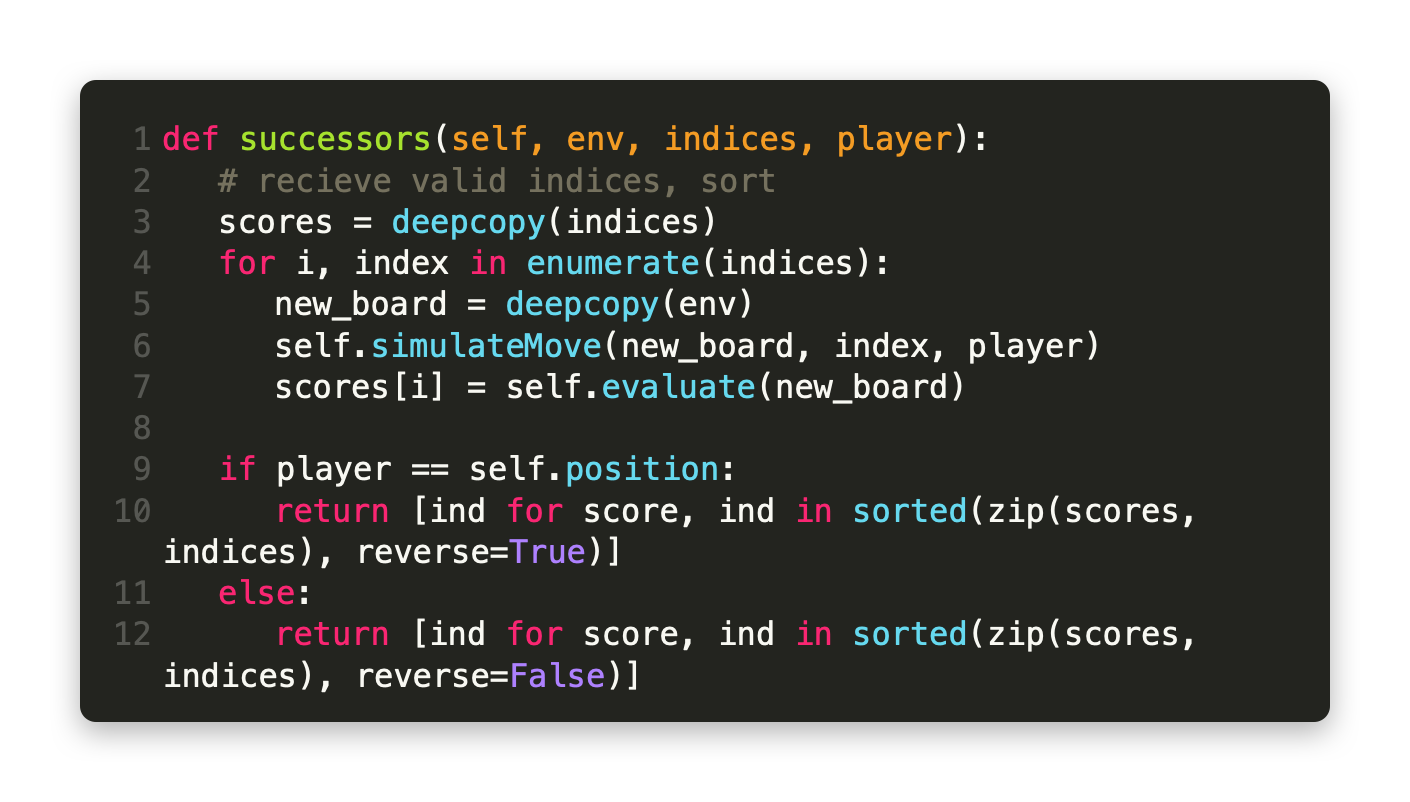
\includegraphics[width = \linewidth]{codye_succ.png}

The successors function takes in the indices list (list of legal moves) and returns the same list, but sorted in order of most promising to least.
For max, this means the indices are returned in nondecreasing order of their evaluation scores. 
For min, this means the indices are returned nonincreasing order of their evaluation scores.

This is helpful because it means we can explore the best nodes first, and unlike Minimax, Alpha Beta pruning will actually take advantage and prune subsequent branches.
As a result, the algorithm should be able to search deeper, at the cost of breadth.

\section{Question 5}

\begin{verbatim}
Alpha Beta Pruning Games

===== AlphaBeta VS MonteCarlo =====

Summary:
p1 Wins: 10
p2 Wins: 0

> python main.py -p1 alphaBetaAI -p2 monteCarloAI -limit_players 1,2 -seed 1
[[0 0 0 1 2 0 0]
 [0 0 0 1 1 0 0]
 [0 0 0 1 1 1 1]
 [0 0 0 2 1 1 2]
 [0 0 1 1 2 2 2]
 [2 0 2 1 2 2 2]]
Player  1  has won

> python main.py -p1 alphaBetaAI -p2 monteCarloAI -limit_players 1,2 -seed 2
[[0 0 2 1 2 0 0]
 [0 0 2 1 1 1 0]
 [0 0 2 1 1 1 0]
 [0 0 1 2 1 2 1]
 [0 0 2 1 2 1 2]
 [2 0 2 1 2 1 2]]
Player  1  has won

> python main.py -p1 alphaBetaAI -p2 monteCarloAI -limit_players 1,2 -seed 3
[[0 0 0 2 2 0 0]
 [0 0 0 1 1 0 0]
 [0 0 2 1 2 0 0]
 [0 1 1 1 1 0 0]
 [2 2 1 2 1 0 0]
 [2 2 1 1 2 0 0]]
Player  1  has won

> python main.py -p1 alphaBetaAI -p2 monteCarloAI -limit_players 1,2 -seed 4
[[0 0 2 1 0 0 0]
 [0 0 1 1 1 0 0]
 [0 0 2 2 1 0 0]
 [0 0 1 1 1 0 0]
 [0 0 2 1 1 0 2]
 [2 0 2 1 2 2 2]]
Player  1  has won

> python main.py -p1 alphaBetaAI -p2 monteCarloAI -limit_players 1,2 -seed 5
[[0 0 1 2 0 0 0]
 [0 0 1 1 0 0 0]
 [0 0 1 2 0 0 1]
 [0 0 1 1 0 0 2]
 [0 0 2 1 0 0 2]
 [0 0 2 1 0 2 2]]
Player  1  has won

> python main.py -p1 alphaBetaAI -p2 monteCarloAI -limit_players 1,2 -seed 6
[[0 0 0 2 0 0 0]
 [0 0 0 1 1 0 0]
 [0 0 0 1 1 0 0]
 [0 0 0 1 1 0 0]
 [0 0 0 2 1 0 2]
 [0 2 0 1 2 2 2]]
Player  1  has won

> python main.py -p1 alphaBetaAI -p2 monteCarloAI -limit_players 1,2 -seed 7
[[0 0 0 0 0 0 0]
 [0 0 0 0 0 0 0]
 [0 0 0 1 0 0 0]
 [0 2 0 1 0 0 0]
 [0 2 0 1 0 0 0]
 [0 2 0 1 0 0 0]]
Player  1  has won

> python main.py -p1 alphaBetaAI -p2 monteCarloAI -limit_players 1,2 -seed 8
[[0 0 2 1 0 0 0]
 [0 0 2 1 0 0 2]
 [0 0 1 2 1 0 1]
 [0 0 1 1 1 2 2]
 [0 0 1 1 1 2 2]
 [0 2 2 1 1 2 2]]
Player  1  has won

> python main.py -p1 alphaBetaAI -p2 monteCarloAI -limit_players 1,2 -seed 9
[[0 0 0 1 2 0 0]
 [2 0 0 1 1 0 0]
 [1 0 2 1 1 0 0]
 [2 0 1 2 1 0 0]
 [2 1 2 1 2 0 0]
 [2 2 1 1 2 0 0]]
Player  1  has won

> python main.py -p1 alphaBetaAI -p2 monteCarloAI -limit_players 1,2 -seed 10
[[0 0 0 1 1 0 0]
 [0 1 0 1 1 0 0]
 [0 1 1 1 2 1 0]
 [0 2 2 2 1 2 1]
 [0 2 1 1 2 1 2]
 [2 2 2 1 2 2 2]]
Player  1  has won

===== AlphaBeta VS MonteCarlo =====

Summary:
p1 Wins: 4
p2 Wins: 6

> python main.py -p1 monteCarloAI -p2 alphaBetaAI -limit_players 1,2 -seed 1
[[0 0 0 0 0 0 0]
 [0 0 0 0 0 0 0]
 [0 0 0 2 0 0 0]
 [0 0 0 2 0 0 0]
 [0 0 0 2 0 0 0]
 [0 1 1 1 1 0 0]]
Player  1  has won

> python main.py -p1 monteCarloAI -p2 alphaBetaAI -limit_players 1,2 -seed 2
[[0 0 0 2 0 0 0]
 [0 0 0 2 1 0 0]
 [0 0 0 1 2 0 0]
 [0 2 1 2 2 0 0]
 [0 1 2 1 1 0 0]
 [0 1 1 2 1 0 0]]
Player  1  has won

> python main.py -p1 monteCarloAI -p2 alphaBetaAI -limit_players 1,2 -seed 3
[[0 0 0 1 0 0 0]
 [0 0 0 2 0 0 0]
 [0 2 2 2 2 0 0]
 [0 1 1 2 2 0 0]
 [0 2 1 1 1 0 0]
 [0 1 1 2 1 0 0]]
Player  2  has won

> python main.py -p1 monteCarloAI -p2 alphaBetaAI -limit_players 1,2 -seed 4
[[0 0 0 2 0 0 0]
 [0 0 0 2 0 2 0]
 [2 0 2 1 0 1 0]
 [1 0 2 2 2 2 0]
 [1 0 1 2 1 1 0]
 [1 0 1 2 1 1 0]]
Player  2  has won

> python main.py -p1 monteCarloAI -p2 alphaBetaAI -limit_players 1,2 -seed 5
[[0 0 2 2 0 0 1]
 [0 0 2 2 0 0 1]
 [0 0 2 2 0 0 2]
 [0 0 2 1 0 0 1]
 [0 0 1 2 0 0 1]
 [1 1 2 1 1 2 1]]
Player  2  has won

> python main.py -p1 monteCarloAI -p2 alphaBetaAI -limit_players 1,2 -seed 6
[[0 0 1 2 0 2 0]
 [0 0 2 2 0 1 0]
 [2 0 2 1 0 1 0]
 [1 0 2 2 1 2 0]
 [1 2 1 1 2 1 0]
 [1 2 1 2 1 1 0]]
Player  1  has won

> python main.py -p1 monteCarloAI -p2 alphaBetaAI -limit_players 1,2 -seed 7
[[0 0 0 0 0 0 0]
 [0 0 0 2 1 0 0]
 [0 0 2 2 2 2 0]
 [0 0 2 1 2 1 0]
 [0 0 1 2 1 1 0]
 [1 2 1 1 1 2 0]]
Player  2  has won

> python main.py -p1 monteCarloAI -p2 alphaBetaAI -limit_players 1,2 -seed 8
[[0 0 0 0 0 0 0]
 [0 0 0 2 0 0 0]
 [0 0 0 2 0 0 0]
 [0 0 0 1 0 0 0]
 [0 0 0 2 2 0 0]
 [0 1 1 1 1 0 0]]
Player  1  has won

> python main.py -p1 monteCarloAI -p2 alphaBetaAI -limit_players 1,2 -seed 9
[[0 0 0 0 0 0 0]
 [0 0 0 2 0 0 0]
 [0 0 2 2 0 0 0]
 [0 0 1 2 0 0 0]
 [0 0 1 2 1 0 0]
 [1 2 1 1 1 2 0]]
Player  2  has won

> python main.py -p1 monteCarloAI -p2 alphaBetaAI -limit_players 1,2 -seed 10
[[0 0 0 0 0 0 0]
 [0 0 0 2 0 0 0]
 [0 0 2 1 0 0 0]
 [0 0 2 2 2 2 0]
 [0 0 1 2 1 1 0]
 [1 2 1 1 1 2 1]]
Player  2  has won
\end{verbatim}

\end{document}